\chapter{Resultados}
\label{chap:resultados}

Neste capítulo seão detalhados os resultados obtidos a partir da aplicação das práticas de laboratório e das respostas do questionário respondido pelos alunos. Além disso, são discutidas as modificações necessárias nas práticas, identificadas durante as aulas de laboratório. 

\section{Resultados do questionário}\label{sec:resultados-dos-questionarios}

O questionário foi aplicado quatro vezes, uma vez após cada prática. Os resultados, analisados para cada categoria de perguntas descritas na Tabela \ref{Tab:questionario}, são mostrados a seguir.

\subsection{Resultados da pesquisa de Q1 e Q2}

Além do conhecimento relacionado à FPGA, os alunos também precisam possuir ou aprender alguns conhecimentos e habilidades no Linux e Amazon EC2 para realizar as tarefas de cada prática de laboratório. Por isso, as duas perguntas fechadas Q1 e Q2 na primeira categoria pede aos alunos que avaliem suas habilidades no Linux e no Amazon EC2, respectivamente. Os estudantes deveriam escolher uma das cinco opções de resposta: sem noção, iniciante, intermediário, avançado e guru total.

Os resultados do questionário referente a essas duas perguntas para cada prática de laboratório são mostrados na Figura \ref{fig:grafico-q1-q2}. Cada coluna mostra a porcentagem de alunos que escolhem cada opção de resposta correspondente a cada prática de laboratório. O nível médio de habilidades em cada prática de laboratório é calculado usando a Fórmula \ref{eq:form-q1-q2} e anotado sob cada grupo de colunas na Figura \ref{fig:grafico-q1-q2}.

\begin{equation}\label{eq:form-q1-q2}
nível \ medio \ de \ habilidades = \sum_{i=0}^{4} (i*porcentagem \ de \ alunos \ classificados \ como \ nivel \ i)
\end{equation}


\begin{figure}[htb!] 
   	    \captionsetup{width=15cm}%Da mesma largura que a figura
		\Caption{\label{fig:grafico-q1-q2} Auto-avaliação do aluno nas habilidades do Linux e do Amazon EC2.}
		\UFCfig{}{
			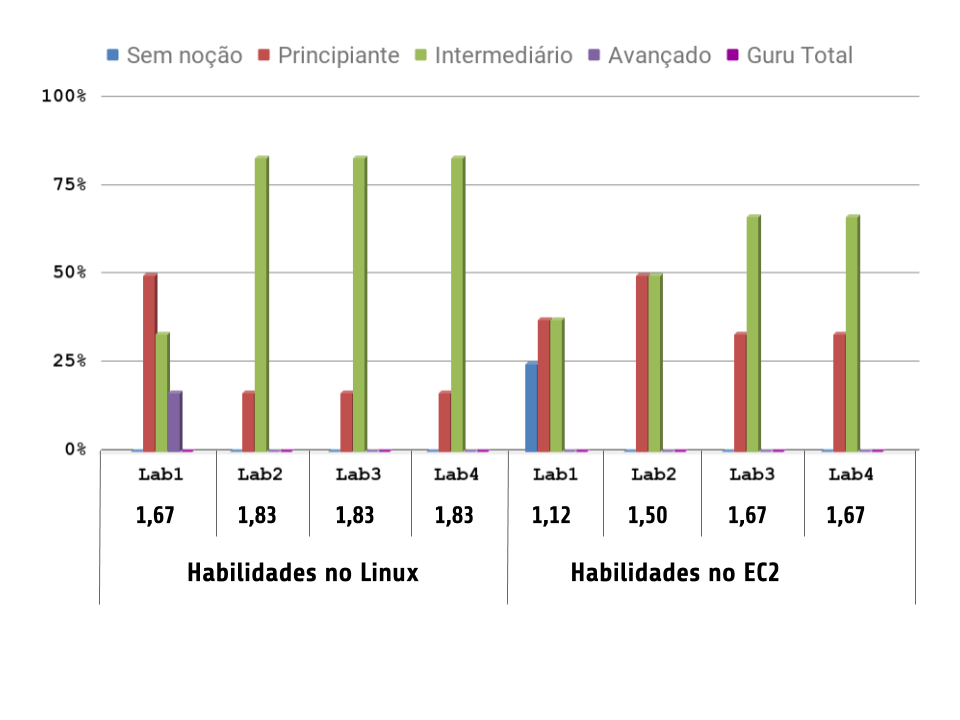
\includegraphics[width=16cm]{figuras/grafico-q1-q2.png}
		}{
			\Fonte{Próprio Autor.}
	}		
\end{figure}

Para obter o nível médio de habilidades, as cinco opções de respostas foram convertidas em valores numéricos, onde o nível 0 significa “Sem noção”, o nível 1 significa “Iniciante”, o nível 2 significa “Intermediário”, o nível 3 significa
“Avançado” e o nível 4 significa “Guru total”. Não existem escalas de intervalo, já que as respostas são ordinais. Essa conversão foi realizada simplesmente para facilitar a comparação dos níveis de habilidades de uma perspectiva relativa, após cada prática de laboratório. 

É possível observar que os exercícios  dessas quatro práticas de laboratório ajudaram o aluno a melhorar suas habilidades de uso do Linux e do EC2. A maioria dos alunos classificaram suas habilidades no Linux como principiante na prática de laboratório 1. O nível médio de habilidades no Linux aumento significativamente da prática de laboratório 1 para a prática de laboratório 2 e se manteve constante até a prática 4.
Em relação ao nível médio de habilidades no EC2, houve um aumento ainda maior da prática de laboratório 1 para a prática de laboratório 2, continuou aumentando para um nível de 1,67 na prática de laboratório 3, até que se manteve constante na prática de laboratório 4. Foi possível perceber que a maioria dos alunos teve alguma experiência no Linux antes de realizar a prática de laboratório 1, e ainda que apesar de todos os alunos terem declarados que não haviam utilizado algum serviço da Amazon Web Services anteriormente, após a prática de laboratório 1 uma porcentagem significativa dos estudantes se classificaram como nível intermediário.


\subsection{Resultados da pesquisa de Q3 e Q4}

Na segunda categoria do questionário estão inclusas duas perguntas fechadas, como mostrado na Tabela \ref{Tab:questionario}. A pergunta Q3 declara que as tarefas em uma prática de laboratório são difíceis. Os estudantes deveriam escolher uma das cinco opções de resposta: discordo fortemente, discordo, nem concordo nem discordo, concordo e concordo fortemente. A pergunta Q4 pede aos alunos para relatar o número de horas que eles gastaram para concluir as tarefas em uma prática de laboratório.

Na Figura \ref{fig:grafico-q3}, cada coluna representa a porcentagem de estudantes que escolheram cada opção de resposta correspondente a cada prática de laboratório em resposta a pergunta Q3. A Figura \ref{fig:grafico-q3eq4} ilustra o nível médio de dificuldade classificado pelos alunos nas tarefas de cada prática de laboratório e o número médio de horas trabalhadas em cada prática de laboratório. O nível médio de dificuldade é calculado usando a fórmula \ref{eq:form-q3}.


\begin{equation}\label{eq:form-q3}
nível \ medio \ de \ dificuldade = \sum_{i=1}^{5} (i*porcentagem \ de \ alunos \ que \ escolheram \ o \ nivel \ i)
\end{equation}



\begin{figure}[htb!] 
   	    \captionsetup{width=15cm}%Da mesma largura que a figura
		\Caption{\label{fig:grafico-q3} Avaliação da afirmação de que as tarefas em uma prática de laboratório são difíceis.}
		\UFCfig{}{
			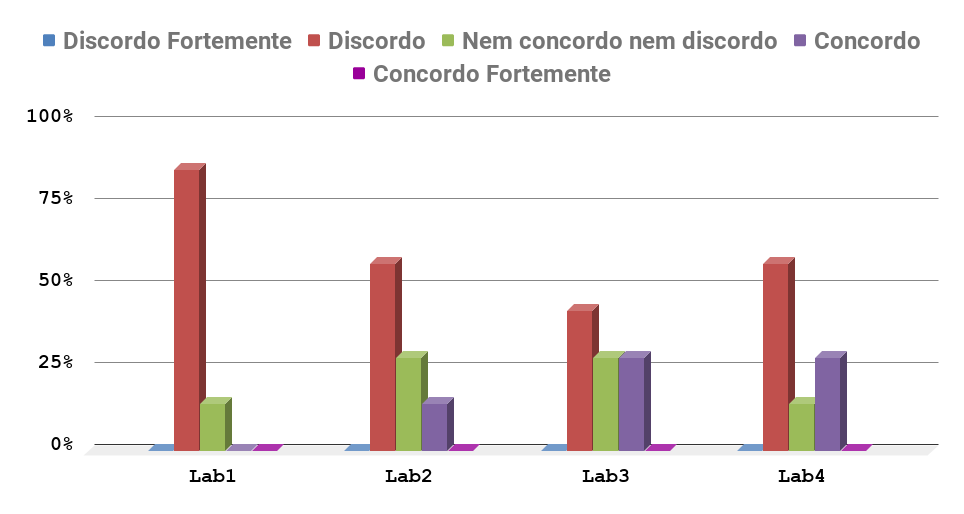
\includegraphics[width=16cm]{figuras/grafico-q3.png}
		}{
			\Fonte{Próprio Autor.}
	}		
\end{figure}

\begin{figure}[htb!] 
   	    \captionsetup{width=15cm}%Da mesma largura que a figura
		\Caption{\label{fig:grafico-q3eq4} Horas trabalhadas e nível médio de dificuldade das tarefas em cada prática de laboratório.}
		\UFCfig{}{
			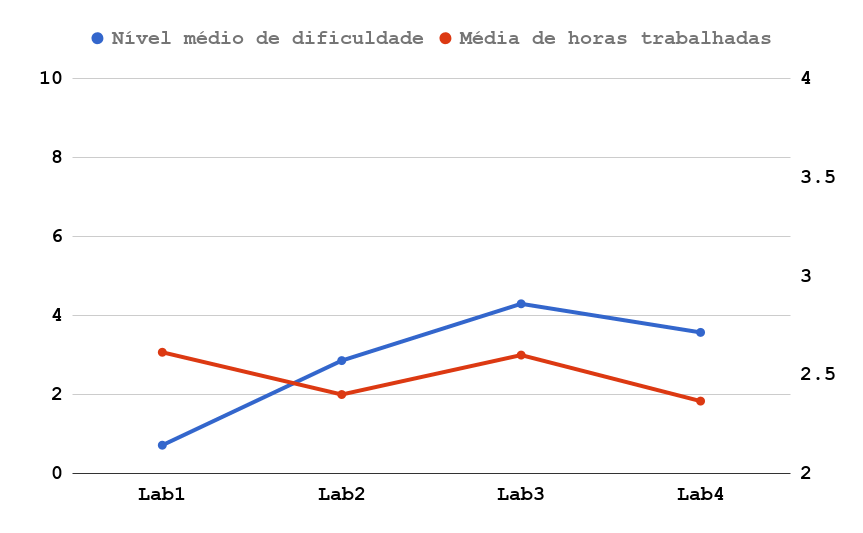
\includegraphics[width=16cm]{figuras/grafico-q3eq4.png}
		}{
			\Fonte{Próprio Autor.}
	}		
\end{figure}

Para obter o nível médio de dificuldade, as cinco opções de respostas foram convertidas em valores numéricos, onde o nível 1 significa “Discordo Fortemente”, o nível 2 significa “Discordo”, o nível 3 significa “Nem concordo nem discordo”, o nível 4 significa “Concordo” e o nível 5 significa “Concordo Fortemente”. Podemos ver na Figura \ref{fig:grafico-q3eq4} que no geral, o número médio de horas gastas pelos alunos em cada prática de laboratório concorda com o nível de dificuldade médio avaliado pelos alunos. O nível médio de dificuldade da prática 1 é menor do que o nível médio de dificuldade da pŕatica 2, contudo menos horas foram gastas no término da prática de laboratório 2. Considerando as curvas de aprendizado das habilidades do Linux e das habilidades do Amazon EC2 ilustradas na Figura \ref{fig:grafico-q1-q2}, essa  inconsistência é razoável, porque os alunos gastaram uma quantidade extra de tempo no aprendizado de Linux e do Amazon EC2. Os resultados também indicam que a prática de laboratório 3 é a mais desafiadora.

\subsection{Resultados da pesquisa de Q5, Q6, Q7 e Q8}

Na terceira categoria, quatro questões Q5, Q6, Q7 e Q8 (conforme a Tabela \ref{Tab:questionario}) foram fornecidas ao alunos para obter suas opiniões sobre o uso da instância EC2 F1. A Figura \ref{fig:grafico-q5-q6-q7-q8} ilustra os resultados obtidos dessas quatro perguntas. Cada coluna representa a porcentagem de estudantes que escolheram a opção de resposta para a pergunta correspondente em cada prática de laboratório, conforme listado na Tabela \ref{Tab:questionario}. O nível médio de concordância com o uso do Amazon EC2 é calculado usando a Fórmula \ref{eq:form-q4-q5-q6-q7-q8} e anotado acima do ID da pergunta, como mostrado na Figura \ref{fig:grafico-q5-q6-q7-q8}. 



\begin{equation}\label{eq:form-q4-q5-q6-q7-q8}
   nível \ medio \ de \ concordância = \frac{1}{4}\sum_{j=1}^{4} (\sum_{i=1}^{5} (i*\Delta)),
\end{equation}
onde $\Delta$ é porcentagem de alunos que escolheram o nível i no lab j.




\begin{figure}[htb!] 
   	    \captionsetup{width=15cm}%Da mesma largura que a figura
		\Caption{\label{fig:grafico-q5-q6-q7-q8} Ranking de concordância com o uso do Amazon EC2.}
		\UFCfig{}{
			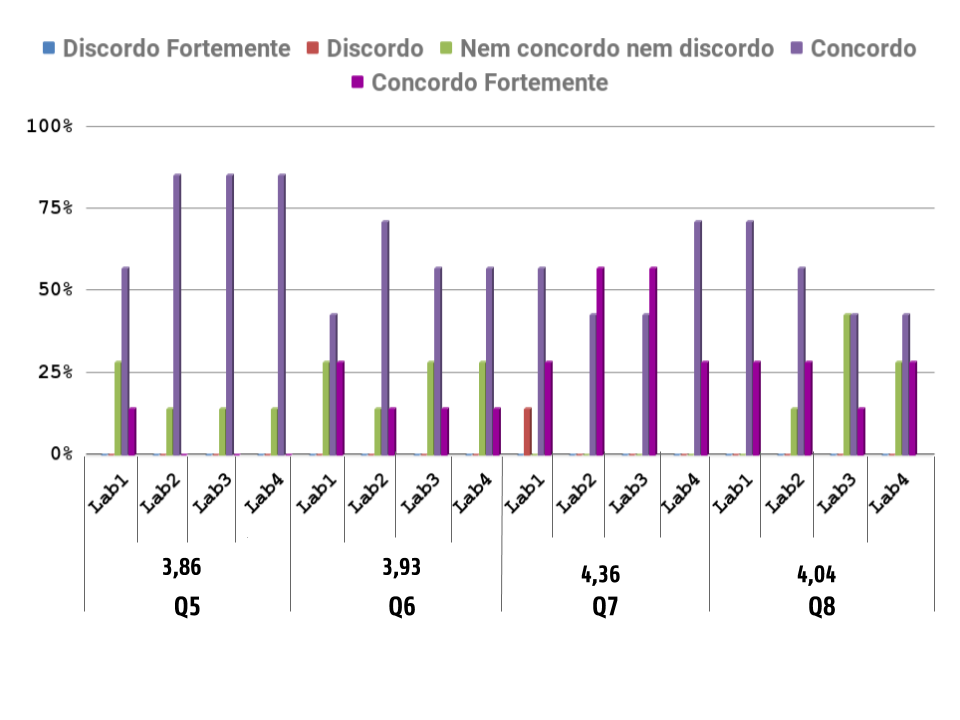
\includegraphics[width=16cm]{figuras/grafico-q5-q6-q7-q8.png}
		}{
			\Fonte{Próprio Autor.}
	}		
\end{figure}

Para obter o nível médio de concordância, as cinco opções de respostas foram convertidas em valores númericos, de maneira idêntica a que foi feita na Fórmula \ref{eq:form-q3}. É possível perceber que a porcentagem de alunos que escolheram a opção "Concordo" permance a mais alta em cada prática de laboratório, exceto para a pergunta Q8 na prática de laboratório 3. Não houveram alunos que escolheram a opção "Discordo fortemente" ou a opção "Discordo", portanto, é possível concluir que a maioria dos alunos  gostaria de usar o Amazon EC2 F1 em exercícios de laboratório de SEDR semelhantes no futuro (Q5), considera a experiência de uso do Amazon EC2 F1  útil para o desenvolvimento de suas carreira (Q6) e usaria o Amazon EC2 F1 em pesquisas/trabalhos no futuro (Q8).

Coom relação à afirmação de que é importante para o aprendizado da disciplina o uso remoto de uma FPGA \textit{high end} (Q7), na primeira prática de laboratório 14,3\% dos alunos discordam com a afirmação, em contra partida, a porcentagem de estudantes que concordam  e concordam fortemente com a afirmação é de 57,1\% e 28,6\%, respectivamente. Além disso, a porcentagem dos alunos que concordam fortemente continua a crescer e não há mais alunos que dicordam nas práticas de laboratório seguintes. Com isso, é possível concluir que a maioria dos estudantes concorda com a importância do uso remoto de uma FPGA  \textit{high end}. 

Quanto à declaração sobre o uso do Amazon EC2 F1 em pesquisas/trabalhos no futuro, 14,3\% dos alunos responderam que nem concordam nem discordam, na prática de laboratório 2, essa porcentagem aumentou para 42,9\% na prática de laboratório 3 e diminuiu para 28,6\% na prática de laboratório 4. Com isso, pode-se dizer que alguns alunos podem ter receio sobre o uso das instâncias EC2 F1 em outras atividades mesmo depois de terem acumulado experiência nas práticas de laboratório. Portanto, acredita-se que uso do Amazon EC2 F1 é benéfico dependendo da natureza da pesquisa ou do trabalho que será realizado.

\subsection{Resultados da pesquisa de  perguntas abertas}

No questionário estão inclusas duas perguntas abertas Q9 e Q10, conforme mostrado na Tabela \ref{Tab:questionario}, a fim de permitir que os alunos comentem abertamente sobre o uso do Amazon EC2 F1 nas práticas de laboratório. A pergunta Q9 trata-se da parte mais difícil para concluir as tarefas em cada prática usando a Amazon EC2. Uma opinião comum indicada pelos comentários dos alunos nas quatro práticas de laboratório é que a falta de experiência com o uso dos comandos necessários para se utilizar o serviço EC2 F1 torna a prática complicada no primeiro momento, mas o uso contínuo dos comandos torna mais fácil a execução das tarefas das práticas de laboratório. Este resultado é consistente com o progresso do nível médio de habilidades no EC2 ilustrado na Figura \ref{fig:grafico-q1-q2}. Três comentários representativos fornecidos pelos alunos à pergunta Q9 são citados diretamente abaixo:


\textit{"A principio, por falta de experiência, o passo a passo é um pouco complicado, mas com o uso fica melhor."}

\textit{"A parte de pedir a instância F1. Mas só porque os comandos são longos e fáceis de confundir. No mais, é tudo muito tranquilo e bem explicado."}

\textit{"Os primeiros contatos com a interface gráfica e a utilização da máquina virtual, o que não foi problemático."}

Houveram alguns comentários negativos em resposta à pergunta Q9, que diz respeito ao tempo disponível para a realização das práticas e a quantidade de tarefas das mesmas. Isso é mostrados nos comentários citados abaixo:

\textit{"Muita atividade e pouco tempo."}

\textit{"Muitas etapas."}

\textit{"Tempo curto."}

É importante destacar alguns comentários específicos da prática de laboratório 4, que mostram que parte da dificuldade de completar as tarefas dessa prática deve-se à falta de recursos computacionais do laboratório para executar a máquina virtual que contém o ambiente de desenvolvimento fornecido pela Amazon Web Services. Alguns desses comentários são citados abaixo:

\textit{"A máquina virtual usada era lenta e alterou alguns valores de endereçamento."}

\textit{"Execução do Vivado em máquinas lentas torna o laboratório desnecessariamente complicado."}

\textit{"A falta de recurso computacional adequado compromete muito a prática."}


A última pergunta Q10 simplesmente pede que os alunos forneçam quaisquer comentários e sugestões sobre cada prática de laboratório em particular e do Amazon EC2 F1. Houveram poucas respostas para essa pergunta, no geral, os alunos ficaram empolgados para exemplos mais complexos na prática de laboratório 1, sugeriram melhoras na descrição da prática e acreditam que com os recursos computacionais adequados tornam as práticas de laboratório 3 e 4 ainda mais interessantes. Três comentários representativos fornecidos pelos alunos na pergunta Q10 são diretamente citados abaixo: 

\textit{"Achei muito interessante. Com a eventual melhora dos laboratório pra fazerem exemplos mais complexos, vai ficar muito bom."}

\textit{"As prática em texto, como todas as práticas de texto aplicadas em qualquer disciplina, são um pouco superficiais, não dando um entendimento completo do que se está fazendo. Uma explanação passo a passo antes da realização da prática seria interessante."}

\textit{"A prática fica legal quando feita com os recursos certos."}

\section{Modificações nas práticas}\label{sec:modificacoes-nas-praticas}

Após a a aplicação de cada prática, percebeu-se a necessidade de algumas alterações nas mesmas. No entanto, foram alterações mínimas, que dizem respeito apenas a modificação do formato dos comandos informados nas práticas, de forma que se tornasse mais intuitivo na hora de usá-los.

